%%%%%%%%%%%%%%%%%%%%%%%%%%%%%%%%%%%%%%%%%
% Beamer Presentation
% LaTeX Template
% Version 1.0 (10/11/12)
%
% This template has been downloaded from:
% http://www.LaTeXTemplates.com
%
% License:
% CC BY-NC-SA 3.0 (http://creativecommons.org/licenses/by-nc-sa/3.0/)
%
%%%%%%%%%%%%%%%%%%%%%%%%%%%%%%%%%%%%%%%%%

%----------------------------------------------------------------------------------------
%	PACKAGES AND THEMES
%----------------------------------------------------------------------------------------

\documentclass{beamer}

\mode<presentation> {

% The Beamer class comes with a number of default slide themes
% which change the colors and layouts of slides. Below this is a list
% of all the themes, uncomment each in turn to see what they look like.

\usetheme{default}
%\usetheme{AnnArbor}
%\usetheme{Antibes}
%\usetheme{Bergen}
%\usetheme{Berkeley}
%\usetheme{Berlin}
%\usetheme{Boadilla}
%\usetheme{CambridgeUS}
%\usetheme{Copenhagen}
%\usetheme{Darmstadt}
%\usetheme{Dresden}
%\usetheme{Frankfurt}
%\usetheme{Goettingen}
%\usetheme{Hannover}
%\usetheme{Ilmenau}
%\usetheme{JuanLesPins}
%\usetheme{Luebeck}
%\usetheme{Madrid}
%\usetheme{Malmoe}
%\usetheme{Marburg}
%\usetheme{Montpellier}
%\usetheme{PaloAlto}
%\usetheme{Pittsburgh}
%\usetheme{Rochester}
%\usetheme{Singapore}
%\usetheme{Szeged}
%\usetheme{Warsaw}

% As well as themes, the Beamer class has a number of color themes
% for any slide theme. Uncomment each of these in turn to see how it
% changes the colors of your current slide theme.

%\usecolortheme{albatross}
%\usecolortheme{beaver}
%\usecolortheme{beetle}
%\usecolortheme{crane}
%\usecolortheme{dolphin}
%\usecolortheme{dove}
%\usecolortheme{fly}
%\usecolortheme{lily}
%\usecolortheme{orchid}
%\usecolortheme{rose}
%\usecolortheme{seagull}
%\usecolortheme{seahorse}
%\usecolortheme{whale}
%\usecolortheme{wolverine}

%\setbeamertemplate{footline} % To remove the footer line in all slides uncomment this line
%\setbeamertemplate{footline}[frame number] % To replace the footer line in all slides with a simple slide count uncomment this line


\setbeamertemplate{navigation symbols}{} % To remove the navigation symbols from the bottom of all slides uncomment this line
}
\usepackage[T1]{fontenc}
\usepackage[utf8]{inputenc}
\usepackage{graphicx}
\usepackage{xcolor}
\usepackage{float}
\usepackage{graphicx} % Allows including images
\usepackage{booktabs} % Allows the use of \toprule, \midrule and \bottomrule in tables
\usepackage{tgheros}
\usepackage[defaultmono]{droidmono}

\usepackage{amsmath,amssymb,amsthm,textcomp}
\usepackage{enumerate}
\usepackage{multicol}
\usepackage{tikz}
\usepackage{sidecap}


\usepackage{listings}

\lstset{
language=C++,
basicstyle=\footnotesize\ttfamily,
keywordstyle=\bfseries\color{blue!60!black},
escapechar=@,
commentstyle=\itshape\color{purple!60!black},
showstringspaces=false,
morekeywords={noexcept,constexpr},
breaklines=true}
%basicstyle=\footnotesize\ttfamily}
%tabsize=4,
%aboveskip={1.0\baselineskip},
%belowskip={1.0\baselineskip},
%showtabs=false,
%showspaces=false,
%prebreak=\raisebox{0ex}[0ex][0ex]{\ensuremath{\hookleftarrow}},
%captionpos=t,
%xleftmargin=\parindent}

% code listing settings
%\lstset{
%    language=C++,
%    basicstyle=\ttfamily\small,
%    aboveskip={1.0\baselineskip},
%    belowskip={1.0\baselineskip},
%    columns=fixed,
%    extendedchars=true,
%    breaklines=true,
%    tabsize=4,
%    prebreak=\raisebox{0ex}[0ex][0ex]{\ensuremath{\hookleftarrow}},
%    frame=L,%lines,
%    showtabs=false,
%    showspaces=false,
%    showstringspaces=false,
%    keywordstyle=\bfseries\color{blue!40!black},%\color[rgb]{0.627,0.126,0.941},
%    commentstyle=\itshape\color{purple!40!black},%\color[rgb]{0.133,0.545,0.133},
%    stringstyle=\color{orange},%\color[rgb]{01,0,0},
%    numbers=left,
%    numberstyle=\small,
%    stepnumber=1,
%    numbersep=10pt,
%    captionpos=t,
%    escapeinside={\%*}{*)}
%}

%\lstdefinestyle{customc}{
%  belowcaptionskip=1\baselineskip,
%  breaklines=true,
%  frame=L,
%  xleftmargin=\parindent,
%  language=C,
%  showstringspaces=false,
%  basicstyle=\footnotesize\ttfamily,
%  keywordstyle=\bfseries\color{blue!40!black},
%  commentstyle=\itshape\color{purple!40!black},
%  identifierstyle=\color{blue},
%  stringstyle=\color{orange},
%}




\bibliographystyle{plain}

%----------------------------------------------------------------------------------------
%	TITLE PAGE
%----------------------------------------------------------------------------------------



\author{Florian Frei} % Your name
\date{\today} % Date, can be changed to a custom date

\begin{document}

% Hello and welcome to my midterm presentation
\title{Midterm presentation}
\subtitle{Adaptive Hierarchical Deep Reinforcement Learning}
\begin{frame}
\titlepage
\end{frame}

\begin{frame}
\frametitle{Motivation}
\includegraphics[scale=0.8]{motivation.pdf}
\end{frame}

\begin{frame}
\frametitle{Option-Critic}
\includegraphics[scale=0.6]{option_critic.pdf}
\end{frame}

\begin{frame}
\frametitle{Termination problem}
\includegraphics[scale=0.6]{option_critic_term_prob.pdf}
\end{frame}

\begin{frame}
\frametitle{Option-Critic with delibration cost}
\includegraphics[scale=0.6]{option_critic_with_cost.pdf}
\end{frame}

\begin{frame}
\frametitle{Problems with Atari}
\includegraphics[scale=0.61]{atari_problem.pdf}
\end{frame}

\begin{frame}
\frametitle{Toy environment}
\includegraphics[scale=0.8]{1d_gridworld.pdf}
\end{frame}

\begin{frame}
\frametitle{Battle of control}
Super policy vs. sub policy (options)
\begin{itemize}
\item[--] option architecture
\end{itemize}
\end{frame}

%%Need delib 0 as comparison?

\begin{frame}
\frametitle{Powerful option}
4 options, 2 layer option, $\epsilon = 0.01$, $delib = 10^{-4}$
\includegraphics[scale=0.2]{./strong/score.png}
\end{frame}

\begin{frame}
\frametitle{Powerful option}
4 options, 2 layer option, $\epsilon = 0.01$, $delib = 10^{-4}$
\includegraphics[scale=0.2]{./strong/activity.png}
\end{frame}

\begin{frame}
\frametitle{Powerful option}
4 options, 2 layer option, $\epsilon = 0.01$, $delib = 10^{-4}$
\includegraphics[scale=0.2]{./strong/termination.png}
-> sub policy in control
\end{frame}


\begin{frame}
\frametitle{Bias option}
4 options, bias option, $\epsilon = 0.01$, $delib = 10^{-4}$
\includegraphics[scale=0.2]{./bias/score_non.png}\\
-> super policy in control\\
-> no convergence
\end{frame}

\begin{frame}
\frametitle{Battle of control}
Super policy vs. sub policy (options)
\begin{itemize}
\item[--] option architecture
\item[--] epsilon $\epsilon$ of super policy
\end{itemize}
\end{frame}

%%Bias option

\begin{frame}
\frametitle{Bias option}
4 options, bias option, $\epsilon = 1.0$ with annealing, $delib = 10^{-4}$
\includegraphics[scale=0.2]{./bias/score.png}
\end{frame}

\begin{frame}
\frametitle{Bias option}
4 options, bias option, $\epsilon = 1.0$ with annealing, $delib = 10^{-4}$
\includegraphics[scale=0.2]{./bias/activity.png}
\end{frame}


\begin{frame}
\frametitle{Future work}
\begin{itemize}
\item[--] l2 regularization on features
\item[--] better feature extraction
\end{itemize}
\end{frame}


\begin{frame}
\frametitle{QnA}
\end{frame}

%\begin{frame}
%\bibliography{ref}
%\end{frame}


\end{document} 